\documentclass[aspectratio=169]{../latex_main/tntbeamer}  % you can pass all options of the beamer class, e.g., 'handout' or 'aspectratio=43'
\usepackage{dsfont}
\usepackage{bm}
\usepackage[english]{babel}
\usepackage[T1]{fontenc}
%\usepackage[utf8]{inputenc}
\usepackage{graphicx}
\graphicspath{ {./figures/} }
\usepackage{algorithm}
\usepackage[ruled,vlined,algo2e,linesnumbered]{algorithm2e}
\usepackage{hyperref}
\usepackage{booktabs}
\usepackage{mathtools}

\usepackage{amsmath,amssymb}

\DeclareMathOperator*{\argmax}{arg\,max}
\DeclareMathOperator*{\argmin}{arg\,min}

\usepackage{amsbsy}
\newcommand{\vect}[1]{\bm{#1}}
%\newcommand{\vect}[1]{\boldsymbol{#1}}

\usepackage{pgfplots}
\pgfplotsset{compat=1.16}
\usepackage{tikz}
\usetikzlibrary{trees} 
\usetikzlibrary{shapes.geometric}
\usetikzlibrary{positioning,shapes,shadows,arrows,calc,mindmap}
\usetikzlibrary{positioning,fadings,through}
\usetikzlibrary{decorations.pathreplacing}
\usetikzlibrary{intersections}
\pgfdeclarelayer{background}
\pgfdeclarelayer{foreground}
\pgfsetlayers{background,main,foreground}
\tikzstyle{activity}=[rectangle, draw=black, rounded corners, text centered, text width=8em]
\tikzstyle{data}=[rectangle, draw=black, text centered, text width=8em]
\tikzstyle{myarrow}=[->, thick, draw=black]

% Define the layers to draw the diagram
\pgfdeclarelayer{background}
\pgfdeclarelayer{foreground}
\pgfsetlayers{background,main,foreground}

% Requires XeLaTeX or LuaLaTeX
%\usepackage{unicode-math}

\usepackage{fontspec}
%\setsansfont{Arial}
\setsansfont{RotisSansSerifStd}[ 
Path=../latex_main/fonts/,
Extension = .otf,
UprightFont = *-Regular,  % or *-Light
BoldFont = *-ExtraBold,  % or *-Bold
ItalicFont = *-Italic
]
\setmonofont{Cascadia Mono}[
Scale=0.8
]

% scale factor adapted; mathrm font added (Benjamin Spitschan @TNT, 2021-06-01)
%\setmathfont[Scale=1.05]{Libertinus Math}
%\setmathrm[Scale=1.05]{Libertinus Math}

% other available math fonts are (not exhaustive)
% Latin Modern Math
% XITS Math
% Libertinus Math
% Asana Math
% Fira Math
% TeX Gyre Pagella Math
% TeX Gyre Bonum Math
% TeX Gyre Schola Math
% TeX Gyre Termes Math

% Literature References
\newcommand{\lit}[2]{\href{#2}{\footnotesize\color{black!60}[#1]}}

%%% Beamer Customization
%----------------------------------------------------------------------
% (Don't) Show sections in frame header. Options: 'sections', 'sections light', empty
\setbeamertemplate{headline}{empty}

% Add header logo for normal frames
\setheaderimage{
	% 
\includegraphics[height=\logoheight]{figures/TNT_darkv4.pdf}
	
\includegraphics[height=\logoheight]{../latex_main/figures/luh_logo_rgb_0_80_155.pdf}
	% 
\includegraphics[height=\logoheight]{figures/logo_tntluh.pdf}
}

% Header logo for title page
\settitleheaderimage{
	% 
\includegraphics[height=\logoheight]{figures/TNT_darkv4.pdf}
	
\includegraphics[height=\logoheight]{../latex_main/figures/luh_logo_rgb_0_80_155.pdf}
	% 
\includegraphics[height=\logoheight]{figures/logo_tntluh.pdf}
}

% Title page: tntdefault 
\setbeamertemplate{title page}[tntdefault]  % or luhstyle
% Add optional title image here
%\addtitlepageimagedefault{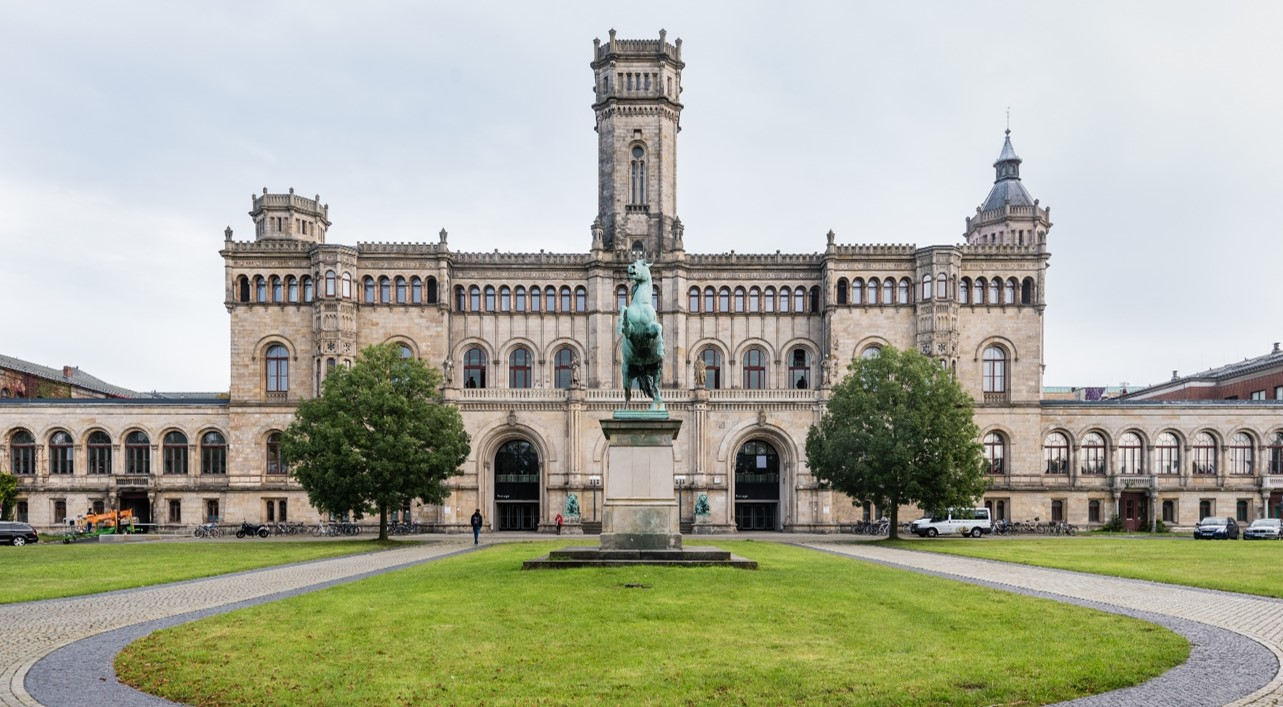
\includegraphics[width=0.65\textwidth]{figures/luh_default_presentation_title_image.jpg}}

% Title page: luhstyle
% \setbeamertemplate{title page}[luhstyle]
% % Add optional title image here
% \addtitlepageimage{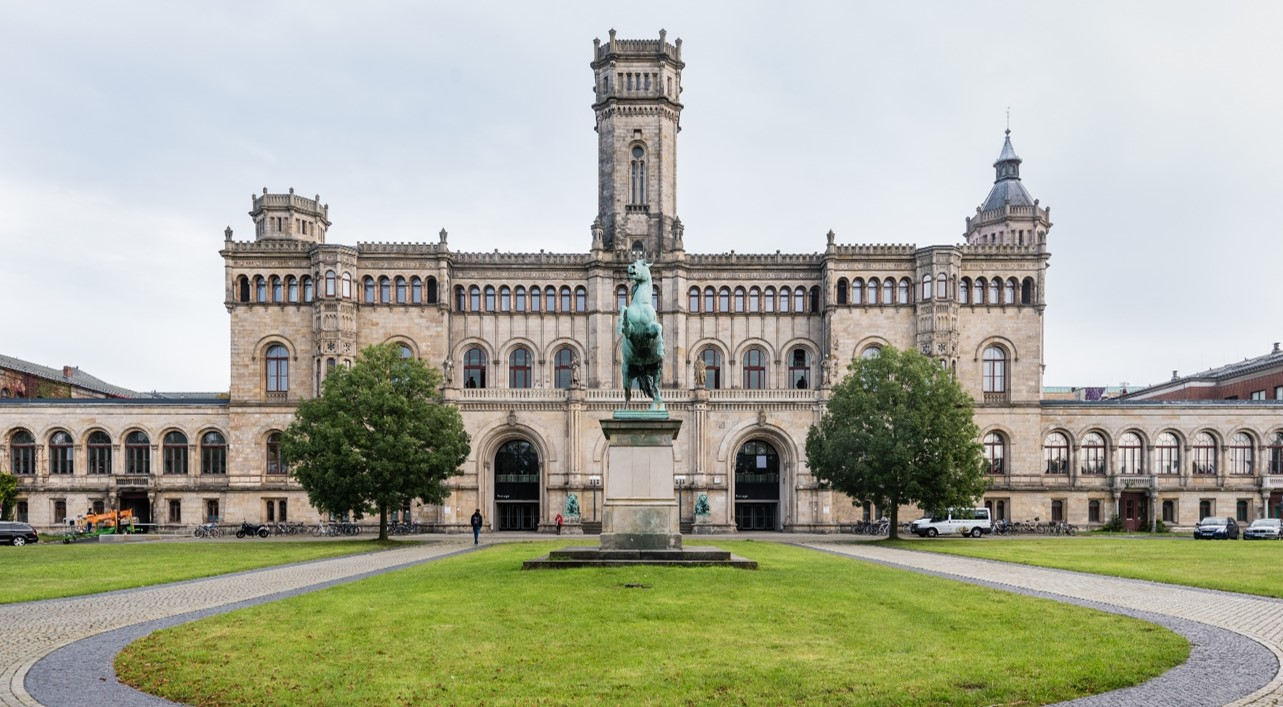
\includegraphics[width=0.75\textwidth]{figures/luh_default_presentation_title_image.jpg}}

\author[Abedjan \& Lindauer]{Ziawasch Abedjan \& Marius Lindauer\\[1em]
	
\includegraphics[height=\logoheight]{../latex_main/figures/luh_logo_rgb_0_80_155.pdf}\qquad
	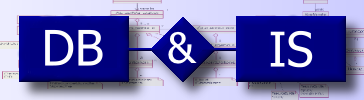
\includegraphics[height=\logoheight]{../latex_main/figures/DBIS_Kurzlogo.png}\qquad

\includegraphics[height=\logoheight]{../latex_main/figures/TNT_darkv4}\qquad

\includegraphics[height=\logoheight]{../latex_main/figures/L3S.jpg}	}
\date{Summer Term 2022; \hspace{0.5em} {
\includegraphics[height=1.5em]{../latex_main/figures/Cc-by-nc-sa_icon.svg.png}}; based on \href{https://ds100.org/fa21/}{[DS100]}
}


%%% Custom Packages
%----------------------------------------------------------------------
% Create dummy content
\usepackage{blindtext}

% Adds a frame with the current page layout. Just call \layout inside of a frame.
\usepackage{layout}


%%% Macros
%\renewcommand{\vec}[1]{\mathbf{#1}}
% \usepackage{bm}
%\let\vecb\bm

\title[Random Forest]{DS: Decision Trees}
\subtitle{Random Forests}

\graphicspath{ {./figure_tree/} }
%\institute{}


\begin{document}
	
	\maketitle
	\begin{frame}[c]{Random Forests: Harnessing Variance}
	    \begin{columns}
	        \begin{column}{.5\textwidth}
	                Fully-grown decision trees will almost always overfit data
	                \begin{itemize}
	                    \item Low model bias, high model variance
	                    \item In other words, small changes in dataset will result in very different decision tree
	                    \item Example: Two models on the right trained on different subsets of the same data
	                \end{itemize}
	                
	                \alert{Random Forest Idea:} Build many decision trees and have them vote
	        \end{column}
	        
	        \begin{column}{.5\textwidth}
	                \begin{figure}
	                    \centering
	                    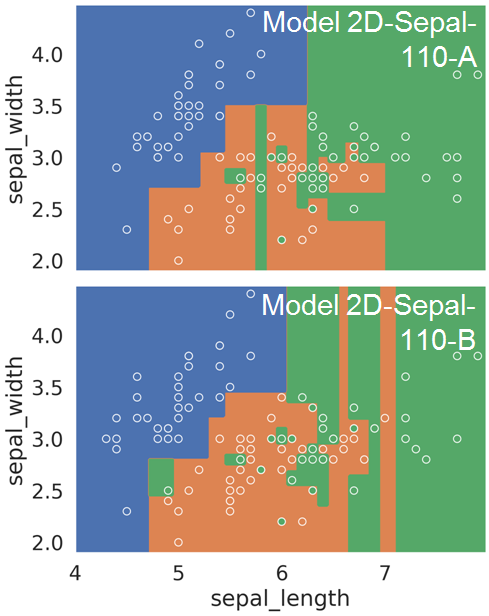
\includegraphics[scale=.35]{Bild55}
	                \end{figure}
	        \end{column}
	    \end{columns}
	\end{frame}
	
	
	\begin{frame}[c]{Random Forests: Harnessing Variance}
	    \begin{columns}
	        \begin{column}{.5\textwidth}
	                What do we mean by vote?
	                \begin{itemize}
	                    \item For a given pair $\bm{x}$, use whichever prediction is most popular
	                \end{itemize}
	                
	                Consider example at right with 9 models
	                \begin{itemize}
	                    \item 6 votes orange, 3 votes green 
	                    \item Random forest prediction is orange
	                \end{itemize}
	        \end{column}
	        
	        \begin{column}{.5\textwidth}
	                \begin{figure}
	                    \centering
	                    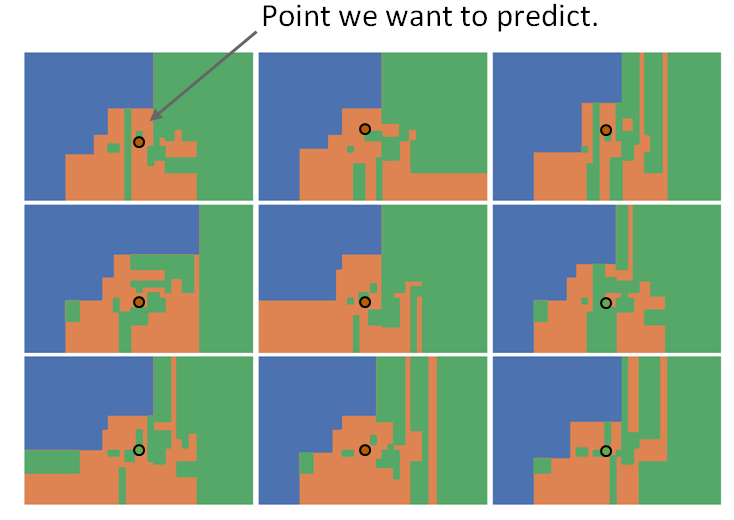
\includegraphics[scale=.35]{Bild56}
	                \end{figure}
	        \end{column}
	    \end{columns}
	\end{frame}
	
	\begin{frame}[c]{Building Many Trees}
	    Big fundamental problem: We only have one training set\\
	    \bigskip
	    How can we build many trees using one training set?

	\end{frame}
	
	
	
	\begin{frame}[c]{Bagging}
	    Bagging: Short for Bootstrap AGGregatING
	    \begin{itemize}
	        \item Generate bootstrap resamples of training data
	        \item Fit one model for each resample
	        \item Final model = average predictions of each small model
	        \item By Leo Breiman in 1994
	        \item Still very well-known model
	    \end{itemize}

	\end{frame}
	
	\begin{frame}[c]{Random Forests}
	    Bagging often isn’t enough to reduce model variance!
	    \begin{itemize}
	        \item Decision trees often look very similar to each other
	        \item E.g., one strong feature always used for first split
	    \end{itemize}
	    
	    \begin{figure}
	        \centering
	        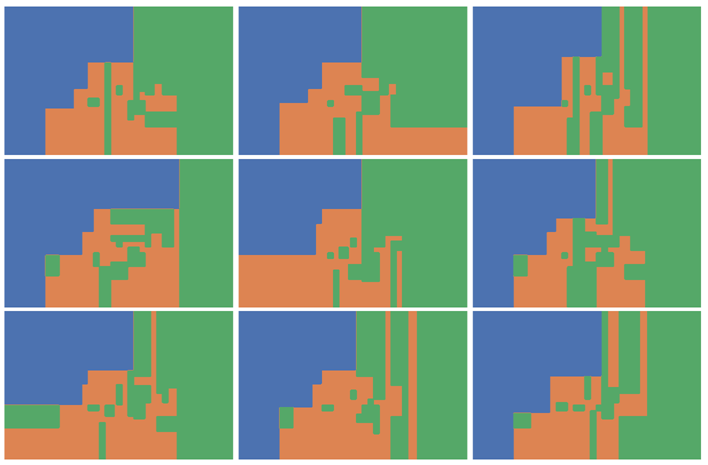
\includegraphics[scale=.4]{Bild57}
	    \end{figure}
	\end{frame}
	
	
	\begin{frame}[c]{Random Forests}
	    \begin{itemize}
	        \item Bagging often isn’t enough to reduce model variance!
	        \begin{itemize}
	            \item Decision trees often look very similar to each other and thus make similar predictions
	            \item Ensemble will still have low bias and high model variance
	            \item E.g. one strong feature always used for first split
	        \end{itemize}
	        \item Idea: Only use a sample of m features at each split
	        \begin{itemize}
	            \item Usually $m = \sqrt{p}$ for decision trees used for classification\footnote{Actually a hyperparameter that can be tuned!}
	            \item Here p is the number of features
	        \end{itemize}
	        \item Algorithm creates individual trees, each overfit in a different way
	        \begin{itemize}
	            \item The hope is that the overall forest has low variance
	        \end{itemize}
	    \end{itemize}
	\end{frame}
	
	\begin{frame}[c]{Random Forests Algorithm Outline}
	    \begin{itemize}
	        \item Bootstrap training data $T$ times.\footnote{Again a hyperparameter!} For each resample, fit a decision tree $t_i$ by doing the following:
	        \begin{itemize}
	            \item Start with data in one node. Until all nodes pure:
	            \begin{itemize}
	                \item Pick an impure node
	                \item Pick a random subset of m features. Pick the best feature x and split value $\beta$ such that the loss of the    resulting split is minimized, e.g. x = petal\_width, $\beta$ = 0.8 has loss 0.66
	                \item Split data into two nodes, one where x < $\beta$, and one where x ≥ $\beta$
	            \end{itemize}
	        \end{itemize}
	        \item To predict, ask the $T$ decision trees for their predictions and take majority vote
	    \end{itemize}
	\end{frame}
	
	\begin{frame}[c]{Avoiding Overfitting with Heuristics}
	    We’ve seen many approaches to avoid overfitting decision trees
	    \begin{itemize}
	        \item Preventing growth
	        \item Pruning
	        \item Random forests
	    \end{itemize}
	    \bigskip
	    These ideas are generally “heuristic”

	    \begin{itemize}
	        \item Not provably best or mathematically optimal
	        \item Instead, they are just ideas that somebody thought sounded good, implemented, then found to work in practice acceptably well
	    \end{itemize}
	\end{frame}
	
	
	\begin{frame}[c]{Why Random Forests?}
	    \begin{itemize}
	        \item Versatile: does both regression and classification
	        \item Invariant to feature scaling and translation
	        \item Automatic feature selection
	        \item Nonlinear decision boundaries without complicated feature engineering
	        \item Doesn’t overfit as often as other nonlinear models (e.g. polynomial features)
	        \item Example of ensemble method: combine the knowledge of many simple models to make a sophisticated model
	        \item Example of using bootstrap to reduce model variance
	    \end{itemize}
	\end{frame}
	
\end{document}